\documentclass[landscape,paperwidth=48in,paperheight=36in,fontscale=0.35]{baposter}
%\documentclass[landscape,a0paper,fontscale=0.35]{baposter}
%\documentclass[paperwidth=48in,paperheight=36in,fontsize=24pt]{baposter}
%\usepackage{geometry}                % See geometry.pdf to learn the layout options. There are lots.
%\geometry{}                   % ... or a4paper or a5paper or ... 
%\geometry{landscape}                % Activate for for rotated page geometry
%\usepackage[parfill]{parskip}    % Activate to begin paragraphs with an empty line rather than an indent
\usepackage{graphicx}
\usepackage{amssymb}
\usepackage{amsmath}
\usepackage{epstopdf}
\usepackage{natbib}
\usepackage{multirow}
\usepackage{setspace}
\usepackage{multicol}
\DeclareGraphicsRule{.tif}{png}{.png}{`convert #1 `dirname #1`/`basename #1 .tif`.png}
\renewcommand\refname{}

%\title{Brief Article}
%\author{The Author}
%\date{}                                           % Activate to display a given date or no date

\begin{document}
\begin{poster}{
 % Show grid to help with alignment
 grid=false,
 % Column spacing
 colspacing=0.7em,
 % Color style
 headerColorOne=cyan!20!white!90!black,
 borderColor=cyan!30!white!90!black,
 % Format of textbox
 textborder=faded,
 % Format of text header
 headerborder=open,
 headershape=roundedright,
 headershade=plain,
 background=none,
 bgColorOne=cyan!10!white,
 headerheight=0.12\textheight,
% headerfont=\scshape\Large,
 headerfont=\textsf\textbf\Large
 }
 % Eye Catcher
 {
     
\includegraphics[width=0.3\textwidth]{dept_ps_lg_hi-res.png}
 }
 % Title
 { \Huge A Bayesian hierarchical sparse factor model for complex experiments in genetical genomics}
 % Authors
 {RJ Cody Markelz\textsuperscript{1}, Sayan Mukherjee\textsuperscript{2}, Daniel Runcie\textsuperscript{3}} %\\[1em]
 {\small{\textsuperscript{1}Department of Plant Biology and \textsuperscript{3}Department of Plant Sciences, UC Davis. \textsuperscript{2}Department of Statistical Science, Duke University}
}
 % University logo
 {
%    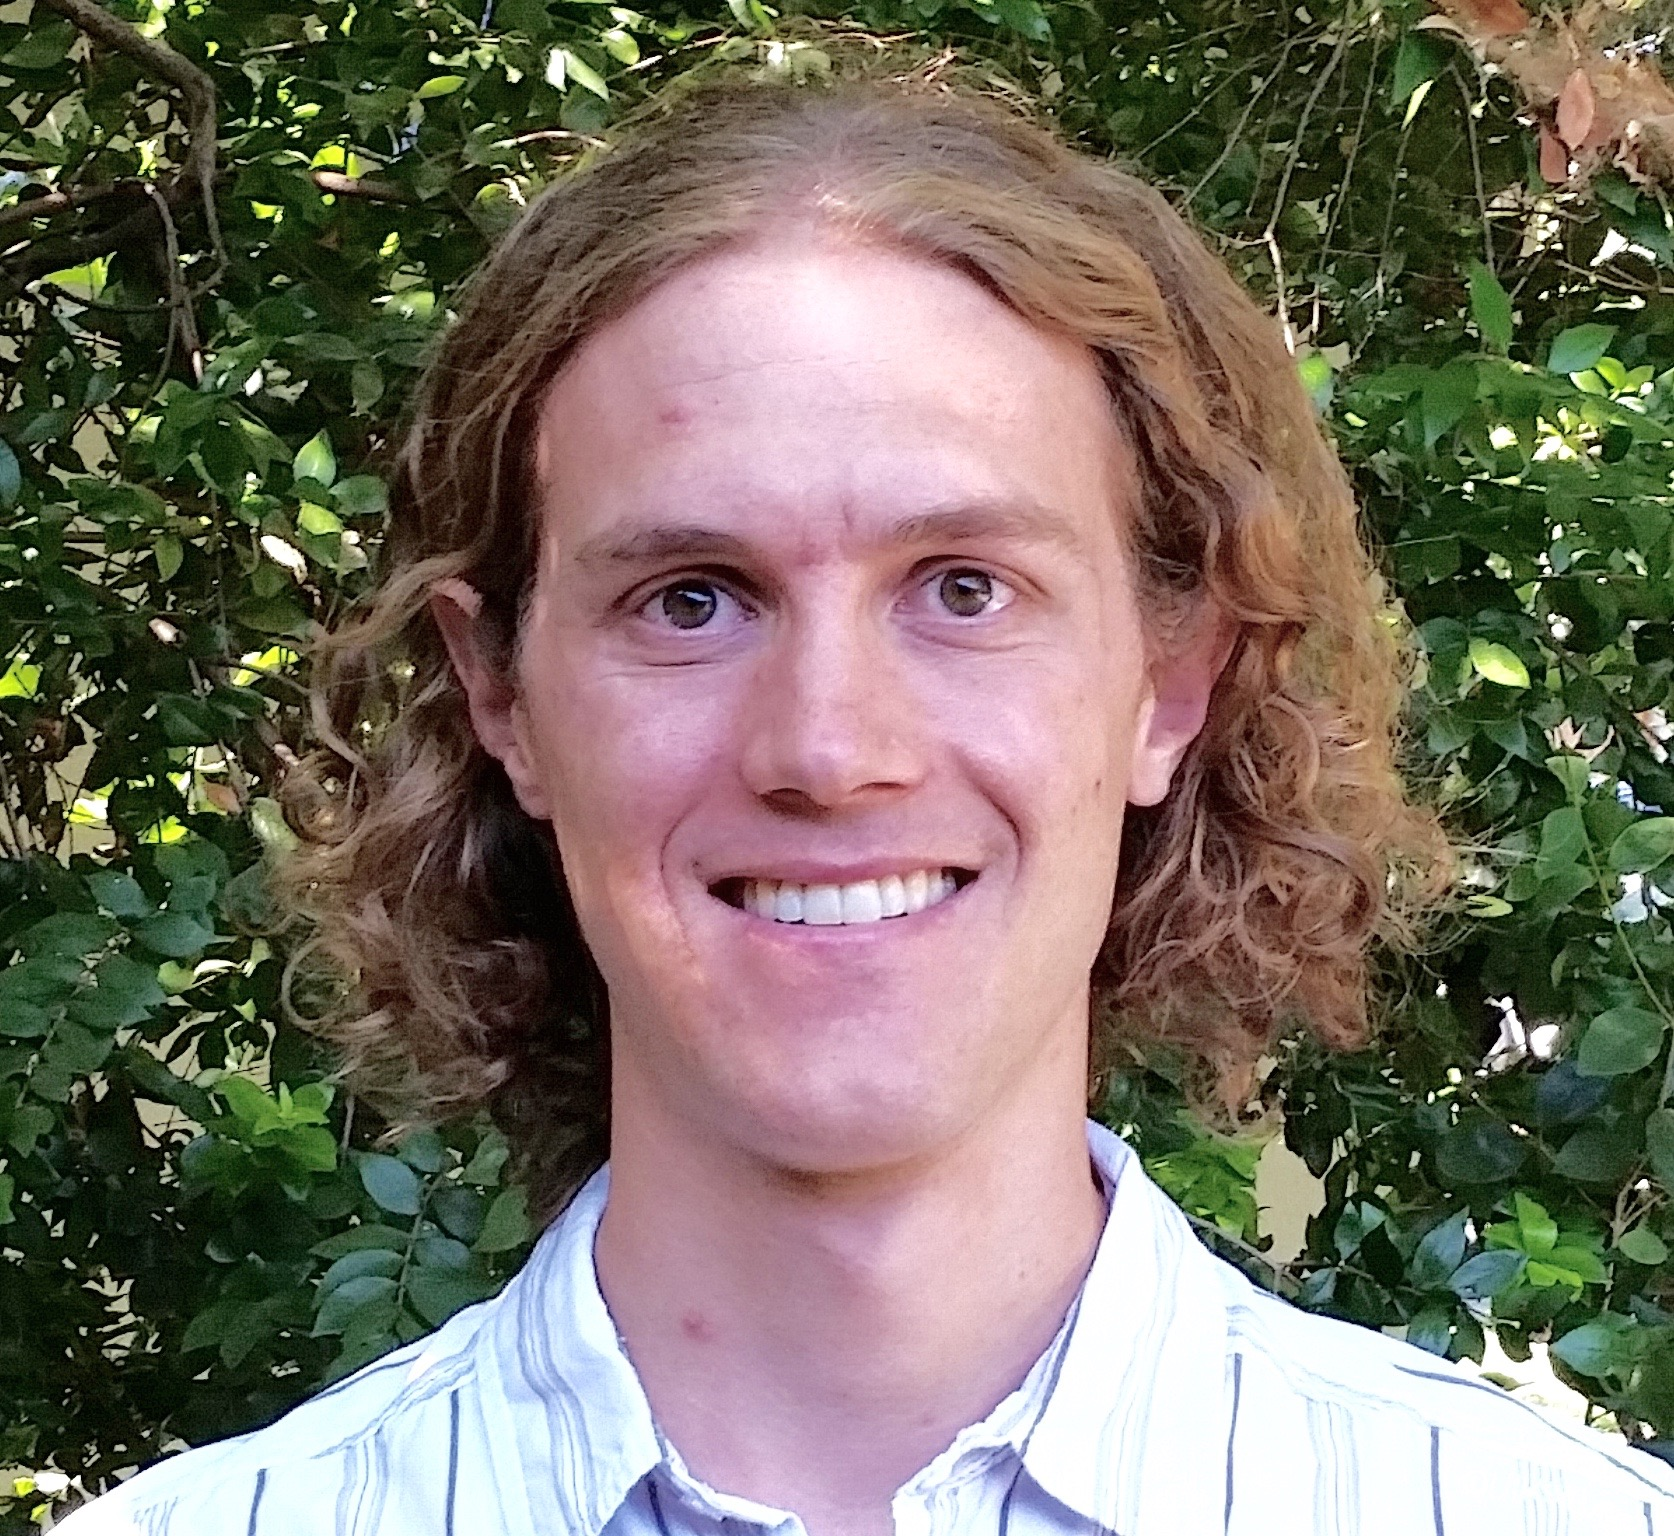
\includegraphics[width=0.05\textwidth]{Runcie_photo.jpg}
 }

%%%%%%%%%%%%%%%%%%%%%%%%%%%%%%%%%%%%%%%%%%%%%%%%%%%%%%%%%%%%%%%%%%%%%%%%%%%%%%
%%% Now define the boxes that make up the poster
%%%---------------------------------------------------------------------------
%%% Each box has a name and can be placed absolutely or relatively.
%%% The only inconvenience is that you can only specify a relative position 
%%% towards an already declared box. So if you have a box attached to the 
%%% bottom, one to the top and a third one which should be inbetween, you 
%%% have to specify the top and bottom boxes before you specify the middle 
%%% box.
%%%%%%%%%%%%%%%%%%%%%%%%%%%%%%%%%%%%%%%%%%%%%%%%%%%%%%%%%%%%%%%%%%%%%%%%%%%%%%

\headerbox{Contribution}{name=a,column=0,row=0,span=2}{
	We present a modeling framework aimed at studying the contributions of genes and the environment to phenotypic variation in high dimensions. Specifically, we are interested in leveraging high-dimensional phenotypes to study the combined effects of multiple factors on traits like yield in crops, fitness in natural populations, or health in patients. Our approach combines two well established principles: 
	\begin{itemize}
	\item Biological systems tend to be modular in organization. 
	\item Complex experimental or breeding designs and observational studies of natural populations with structure require flexible hierarchical models.
%	\item That appropriately designed and analyzed experiments are necessary to address complex experimental questions.
	\end{itemize}

Building on our earlier genetic sparse factor model \citep{Runcie:2013ky}, we extend the specification to allow a full linear mixed effect model to capture complex experimental designs. Using an efficient Bayesian MCMC algorithm, the model scales well both computationally and numerically to dimensions relevant to modern phenotype-centric datasets and generates descriptions of modules that are interpretable with respect to the environmental or genetic factors. 
}

\headerbox{Motivation}{name=b,column=0,below = a}{
%	Technological advances are leading to a revolution in the collection of phenotype data - from the various *seq technologies (ex RNAseq, ChIPseq, DNase-Seq), to proteomics, metabalomcs, and 3D and hyperspectral imaging. 
	High-dimensional phenotypes (ex RNAseq, metabalomcs,  hyperspectral imaging) promise to provide an unprecedented window into the complex functions of biological organisms. 
Settings we have in mind include:
\begin{itemize}
\item A set of genetically related individuals assigned to 2+ treatments to assess gene-environment interactions.
% and then a large set of traits (such as gene expression) are measured on each individual simultaneously. 
\item Multi-factor experiments with split-plot or repeated measures designs that are common in agriculture settings.
\item Case-control studies with individuals of varying ancestry. 
\end{itemize}
	
	In each case the experimental goals are to identify sets of traits associated with each experimental factor and to understand the biological bases of these effects.
}
\headerbox{Analytical challenges}{name=c,column=1,below = a}{
	In these examples, the analytical challenges are a combination of those that affect univariate quantitative genetic analyses and those that affect the study of high dimensional data:
\begin{itemize}
\item Individuals within (and across) treatments are correlated due to shared genetic history.
\item Interactions (ex. Genotype x Treatment) greatly increase the number of parameters for each trait.
\item Traits are correlated and may be functionally related
\item The number of traits (and between-trait covariances) may be larger than the number of individuals ($n << p$)
\end{itemize}
}
\headerbox{Approach} {name=d,column=0,below = b,span=2}{
We view the high-dimensional phenotype as a readout of a modular and time-ordered developmental process (Figure 1). 

This model has the following implications:
\begin{itemize}
\item Experimental factors (genotypes, treatments) cause perturbations to the modules of the developmental system.
\item The traits we observe are independent conditional on the state of the underlying developmental system.
%\item We cannot directly observe the modules, but can indirectly identify them based on a) the correlation they induce among traits in each individual, and b) the correlation of modules across individuals induced by the experimental design and the genetic structure in the population.
\item The same module might explain responses to multiple experimental factors (Figure 2).
\end{itemize}

We therefore focus on identifying the most important modules, which we assume will account for the majority of the effect of the experimental factors on the downstream high-dimensional phenotype. 

\begin{multicols}{2}
\begin{center}
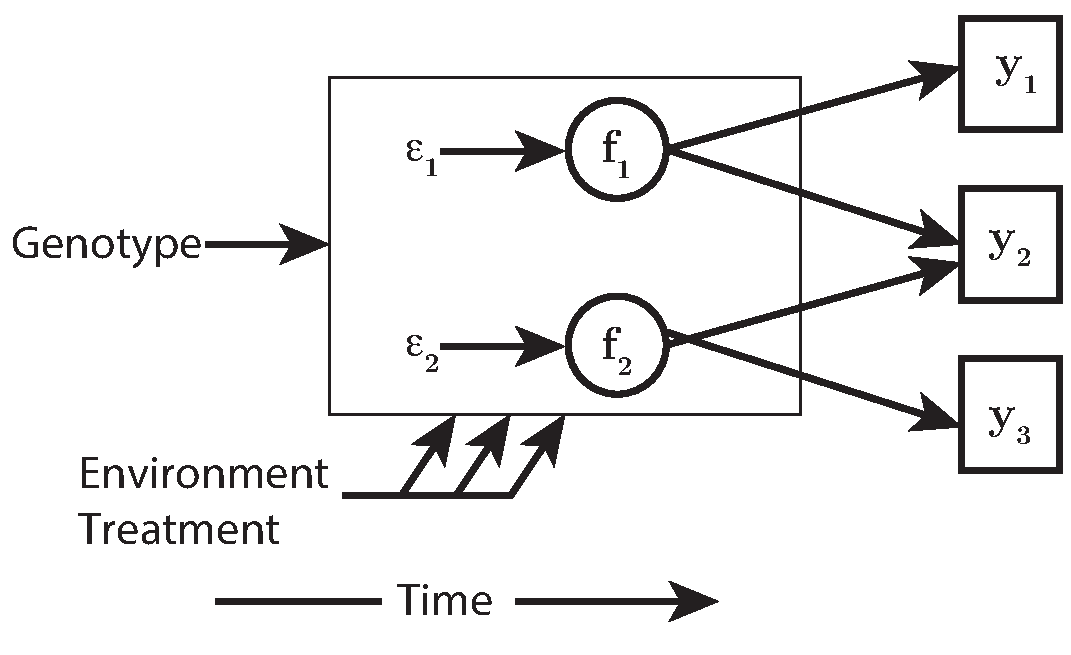
\includegraphics[width=0.825\columnwidth]{Figure1.pdf} 
\end{center}
\textbf{Figure 1.} We assume that the influence of genotype and treatment on the observed traits $\mathbf{y}_j$ is mediated through developmental modules $\mathbf{f}_l$.
\newpage
\begin{center}
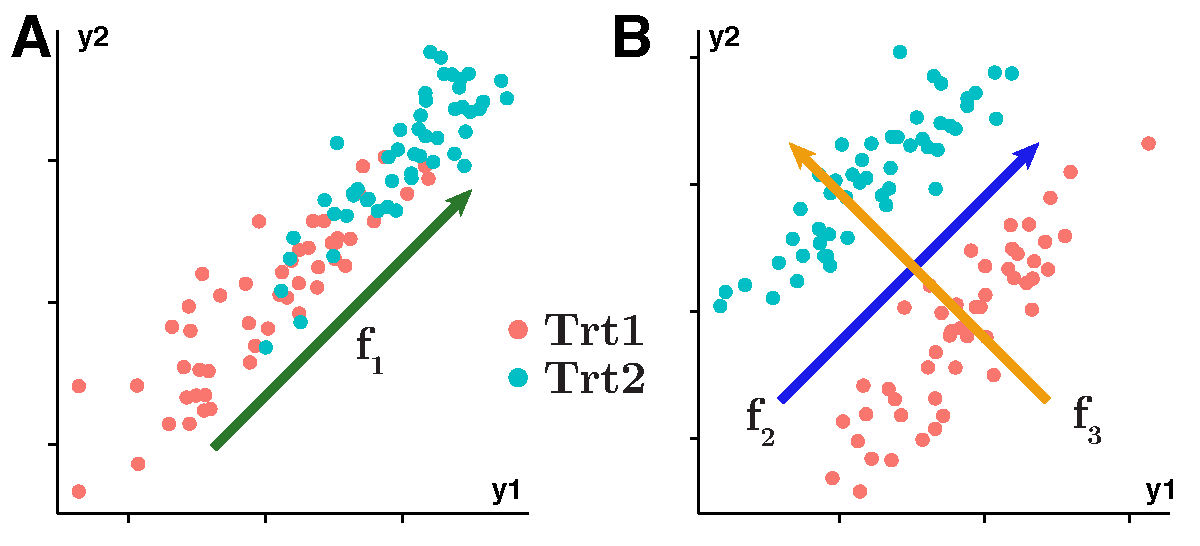
\includegraphics[width=1\columnwidth]{Figure2.pdf} 
\end{center}
\textbf{Figure 2.} When treatment and residual correlations align (as in \textbf{A} but not \textbf{B}) the same factor can explain variation in both traits.
\end{multicols}
}
\headerbox{Model specification} {name=e,column=2,row=0,span=1}{
\subsection*{Sparse factor model}
Motivated by the conceptual model in Figure 1, we model the $n \times p$ phenotype matrix $\mathbf{Y}$ with a sparse factor model, with $k$ factors representing latent developmental modules:
\begin{align}
%\mathbf{Y} &= \mathbf{F}\mathbf{\Lambda}' + \mathbf{E}
\mathbf{Y} &= \mathbf{f}_1\pmb{\lambda}'_1 + \mathbf{f}_k\pmb{\lambda}'_k + \dots \mathbf{f}_k\pmb{\lambda}'_k + \mathbf{E}
\end{align}
Conditional on the factors, the residuals (rows of $\mathbf{E}$) are independent and assigned Gaussian priors.
%Sparsity is induced on the elements of the loadings matrix $\mathbf{\Lambda}$ with the infinite factor model of \citep{Bhattacharya:2011gh} which uses both global shrinkage on each column $\mathbf{\lambda}_{.l}$ through $\tau_l$ and local shrinkage on each element $\lambda_{jl}$ through $\psi_{jl}$. Importantly, a prior on the sequence $\{\tau_1\; \tau_2 \; \dots \tau_k\}$ that biases towards increasing values (more shrinkage) for higher index columns is induced by with a hierarchical structure:
Sparsity in the factor loadings $\pmb{\lambda}_l$ is induced with an ``infinite factor"\citep{Bhattacharya:2011gh} prior structure, using local/global shrinkage with increasing shrinkage on higher-indexed factors. This induces a ranking of the factors and reduces the burden of pre-selecting the number of factors.
\begin{align}\begin{split}
\lambda_{jl} &\sim \mbox{N}(0,\tau^{-1}_k \psi^{-1}_{jl}) \quad \psi_{jl} \sim \mbox{Ga}(\nu/2,\nu/2) \\
\delta_1 &\sim \mbox{Ga}(\alpha_0,\beta_0)\quad \delta_l \sim \mbox{Ga}(\alpha_1,1) \quad 
\tau_l = \prod_{i=1}^k \delta_l
\end{split}\end{align}

\subsection*{Mixed Effect Model (MEM)}
Vectors $\mathbf{f}_l$ represent trait values across the $n$ individuals for each of the $k$ latent modules. We assume that each module is independent and model its variation with a linear mixed effect model:
\begin{align}
\mathbf{f}_{l} &= \mathbf{X} \beta_l + \mathbf{Z}_1 \mathbf{a}_{1l} + \mathbf{Z}_2 \mathbf{a}_{2l} + \boldsymbol{\epsilon}_l \\
\beta_l &\sim \mbox{N}_b(\mathbf{0},\sigma^2_{b_l} (\mathbf{X}'\mathbf{X})^{-1}) &&\mbox { Treatment effect} \nonumber \\
\mathbf{a}_{1l} &\sim \mbox{N}_r(\mathbf{0},\sigma^2_{a_{1l}} \mathbf{A}), \mathbf{a}_{2l} \sim \mbox{N}_r(\mathbf{0},\sigma^2_{a_{2l}} \mathbf{A}) 
	&&\mbox { G and GxT effects}  \nonumber \\
\mathbf{\epsilon}_l &\sim \mbox{N}_r(\mathbf{0},\sigma^2_{e_l} \mathbf{I}) &&\mbox { Residual variation}  \nonumber \\
&\sigma^2_{b_l} + \sigma^2_{a_{1l}} + \sigma^2_{a_{2l}} + \sigma^2_{e_l} = 1
\end{align}


\subsection*{Summary}
The key features of this specification are:
\begin{itemize}
%\item We only describe a single ``fixed" (\emph{e.g.} experimental factor) and a single random (\emph{e.g.} genetic group) factor here, but others (\emph{e.g.} GxE interaction) are added similarly.
\item Specifying the MEM for $\mathbf{f}_l$ instead of $\mathbf{y}_j$ is a massive reduction of complexity because the number of traits is small $k << p$ and the latent traits are assumed uncorrelated.
\item While factors with shared genetic, treatment and residual components are preferred (Figure 2), purely residual factors are allowed.
%We place a simplex prior on the balance among the variance components as a simplex to constrain the total variance of each column (Figure XX). 
\item Given a small $k$, not all variation may be accounted for by the latent factors. We model each trait's residual vector (row of $\mathbf{E}$) with a parallel MEM, and place an additional prior $\pi_j$ on the proportion of variation in that trait accounted for by the $k$ factors.
\end{itemize}
\subsection*{Implementation}
We use a Gibbs sampler implemented in R/Rcpp to estimate the posterior distribution of all model parameters and also coded the model in Stan\citep{Carpenter:2015}.

}

\headerbox{Acknowledgements} {name=g,column=2,below = e}{
We would like to thank Upendra K Devisetty and Julin Maloof for sharing the gene expression data, NSF grants DMS-1418261 and IIS 1546331 to SM and IOS-1402495 to RJCM and the UC Davis Department of Plant Sciences for funding.
}

\headerbox{Data example} {name=f,column=3,row=0,span=1}{
\subsection*{Background}

\begin{multicols}{2}
When plants grow in close proximity to one another they alter their development and physiology to compete for light at the top of the canopy having negative consequences on final yield. This response is regulated through the shade avoidance pathway involving a large gene network of transcription factors, hormone biosynthesis genes and metabolic genes. We have subset a large genetical genomics dataset collected on a recombinant inbred line (RIL) population of $Brassica$  $rapa$ grown in either crowded or uncrowded conditions in the field to examine known shade avoidance genes [Kazu reference]. 
\newpage
\begin{center}
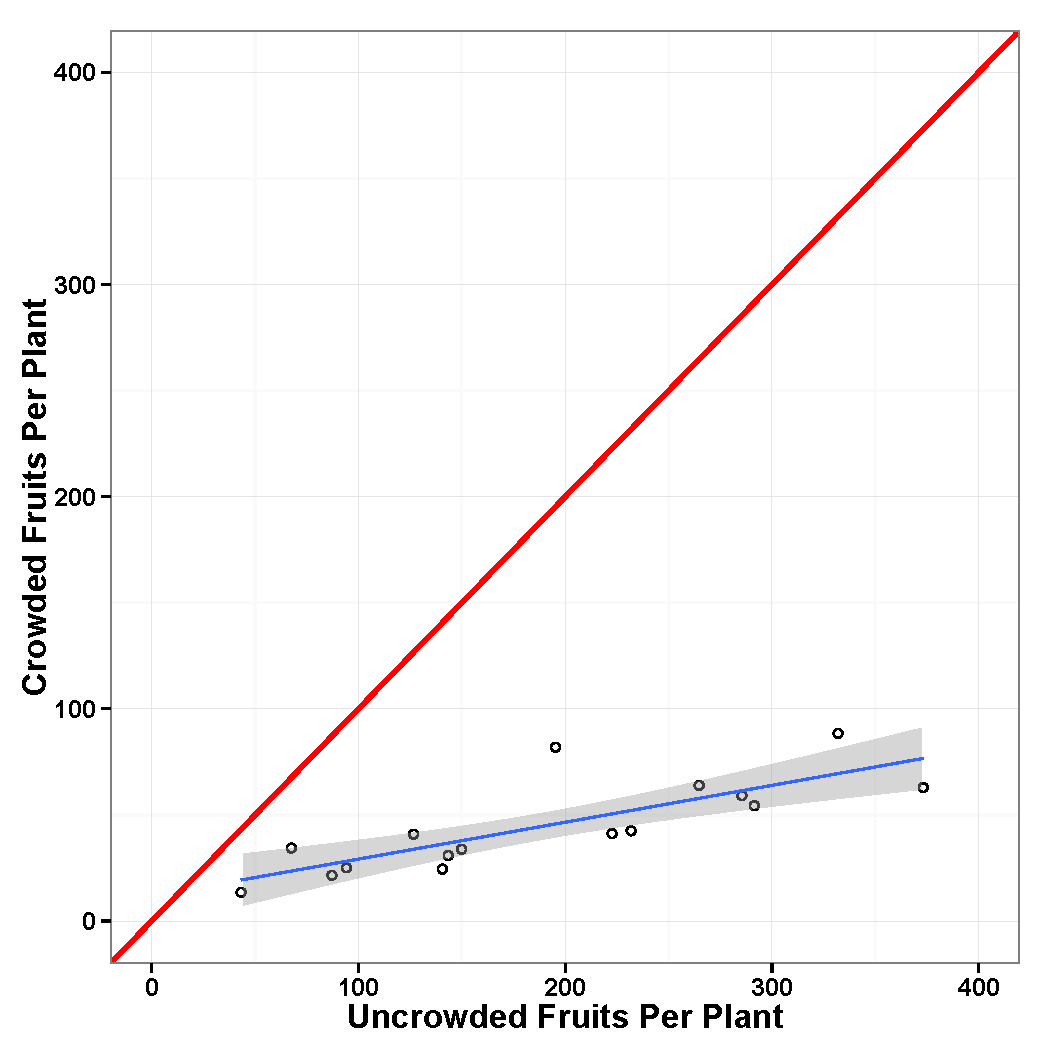
\includegraphics[width=1\columnwidth]{UN_CR_Fruit_regression.pdf} 
\end{center}
\textbf{Figure 4.} Comparison of per plant fruit number on a subset of genotypes from the $Brassica$  $rapa$ RIL population grown in crowded or uncrowded field conditions.
\end{multicols}

\subsection*{Results}

\begin{multicols}{2}
Our model identified five large factors that accounted for the majority of the covariance in the data. 
Interestingly, the two genes that have the greatest positive factor loadings for factor three are PHYA (PHYTOCHROME A) a photoreceptor gene involved in shade detection, and a gene that regulates expression of PHYA, SPA (SUPPRESSOR OF PHYA). 

The factor loadings for factor one include a top positive loading gene, TAA1 (TRYPTOPHAN AMINOTRANSFERASE OF ARABIDOPSIS 1), an auxin biosynthesis gene, and a top negative loading gene, PIN3 (PIN-FORMED 3), is an auxin transport gene. 

These modeling results are promising that the loadings explaining either large genetic or treatment effects are selecting known subnetworks involved in the shade avoidance pathway.
\newpage
\begin{center}
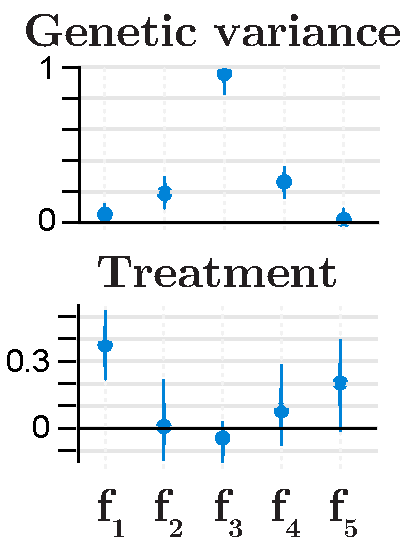
\includegraphics[width=1\columnwidth]{Figure_factors2.pdf} 
\end{center}
\textbf{Figure 5.} Among-line genetic variance and response to crowded conditions for each of the five major factors.
\end{multicols}
}
\headerbox{References} {name=g,column=3,below=f,span=1}{
\bibliography{All_refs}
\bibliographystyle{plain}
% kazu's paper is here. 
% http://journals.plos.org/plosgenetics/article?id=10.1371/journal.pgen.1004953
}

\end{poster}

\end{document}  